\documentclass[16pt]{article}
\usepackage[a4paper, left=1 cm, right=1cm, top=0.5cm, bottom=1cm] {geometry}
\date{} % Remove a exibição da data
\usepackage{xcolor}
\usepackage{listings}
\usepackage{graphicx}
\usepackage[utf8]{inputenc}
\usepackage[T1]{fontenc}


\title{inglês}
\begin{document}
\maketitle
\section{modais}
\textbf{
  Caracteristicas
}
\begin{figure}[htbp]
  \centering
  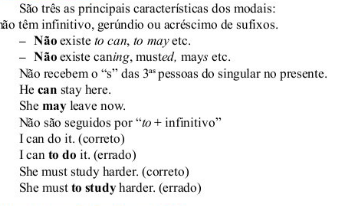
\includegraphics[width=0.5\textwidth]{carac.png}
  \caption{caracteristicas dos modais}
\end{figure}


\subsection{can could}
can = simple present\\
could = simple past
\begin{figure}[htbp]
  \centering
  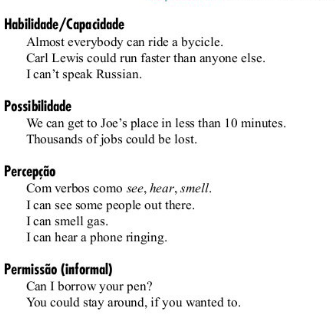
\includegraphics[width=0.5\textwidth]{can-could.png}
  \caption{aplicações}
\end{figure}

\begin{figure}[htbp]
  \centering
  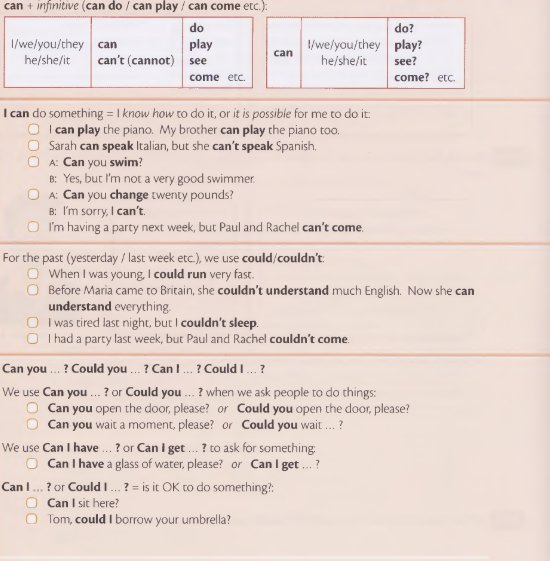
\includegraphics[width=1.0\textwidth]{prin.png}
  \caption{}
\end{figure}

\subsection{may  might}
may = simple present\\
might = simple pass
\begin{figure}[htbp]
  \centering
  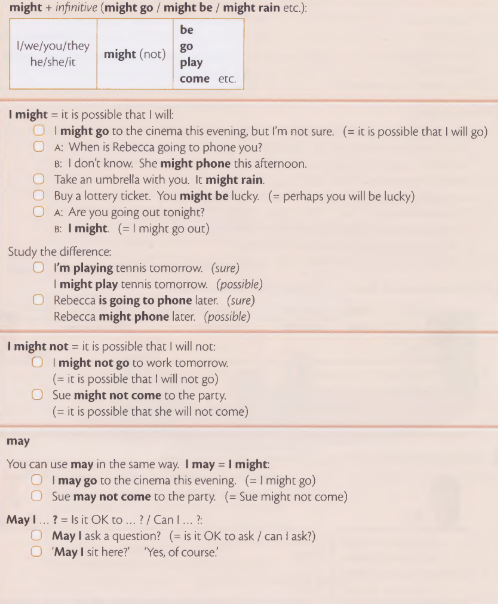
\includegraphics[width=1.0\textwidth]{might.png}
  \caption{}
\end{figure}












\end{document}